\chapter{Projeto do Algoritmo Recursivo}
\label{cap:recursivo}

\section{Introdução}

Neste capítulo, será introduzido um novo algoritmo para encontrar os conjuntos de enlaces viáveis em uma rede sem fio. Esse algoritmo é baseado nos mesmos modelos apresentados no Capítulo \ref{cap:modelagem}, portanto ele possui algumas similaridades como o Algoritmo Iterativo introduzido no Capítulo \ref{cap:iterativo}. 

Como será mostrado nas próximas seções, o diferencial consiste em uma nova maneira de percorrer a árvore, que permitirá que os cálculos da SINR dos enlaces em uma dada combinação sejam reutilizados por seus descendentes. Finalmente, o algoritmo será detalhado e sua complexidade analisada.

\section{Percorrendo a Árvore Recursivamente}

A grande diferença com relação ao Algoritmo Iterativo está na forma em que a árvore é percorrida. No caso iterativo, faz-se uma contagem, ou seja, visita-se os vértices da árvore somando 1 ao seu valor codificado anterior. O caso recursivo não é tão simples e essa seção será dedicada ao seu entendimento.

Como foi mencionado no capítulo anterior, é possível saber quantos descendentes tem um conjunto codificado $B$. Para isso, basta encontrar o {\it bit} ativo menos significativo $b_i^*$ (o {\it bit} 1 mais à direita) e o número de {\it bits} 0 depois de $b_i^*$ é o número de filhos de $B$. Como consequência disso, é possível notar que as folhas da árvore possuem os seus {\it bits} menos significativos ativos, ou seja, se $B$ é ímpar, então $B$ é folha. Um caso especial surge ao analisar $B=0$. Nesse caso, não existem {\it bits} ativos e, por convenção, o número de filhos de $B=0$ é $|B|$.

Além de saber quantos filhos tem a combinação $B$, conhecer $b_i^*$ também nos permite alcançar os filhos de $B$. Para adicionar mais um enlace em $C$ e, com isso, descobrir um possível filho de $B$ na árvore, basta que um dos {\it bits} 0 depois de $b_i^*$ seja alternado para 1. De maneira geral, para fazer essa alternância, basta realizar a soma $B + 2^i$, tal que, $i < i^*$. Consequentemente, para alcançar todos os filhos de uma combinação B basta fazer $B + 2^i$, $\forall i$, tal que, $0\leq i\leq i^*$. Portanto, uma pequena contagem é feita para alternar todos os {\it bits} 0 depois de $b_i^*$ em uma combinação $B$ com o intuito de encontrar os filhos de $B$.

De maneira análoga, os netos de $B$ podem ser encontrados por meio da aplicação da técnica descrita nos filhos de $B$. Em geral, para encontrar todos os descendentes de uma combinação $B$, basta aplicar recursivamente a técnica em cada descendente de $B$. Quando a recursão alcançar uma folha, essa instância se encerra. Se a técnica descrita for aplicada para $B=0$, então todos os seus descendentes serão alcançados e, portanto, toda a árvore de combinações será visitada. 

\begin{figure}[htb]
\centering
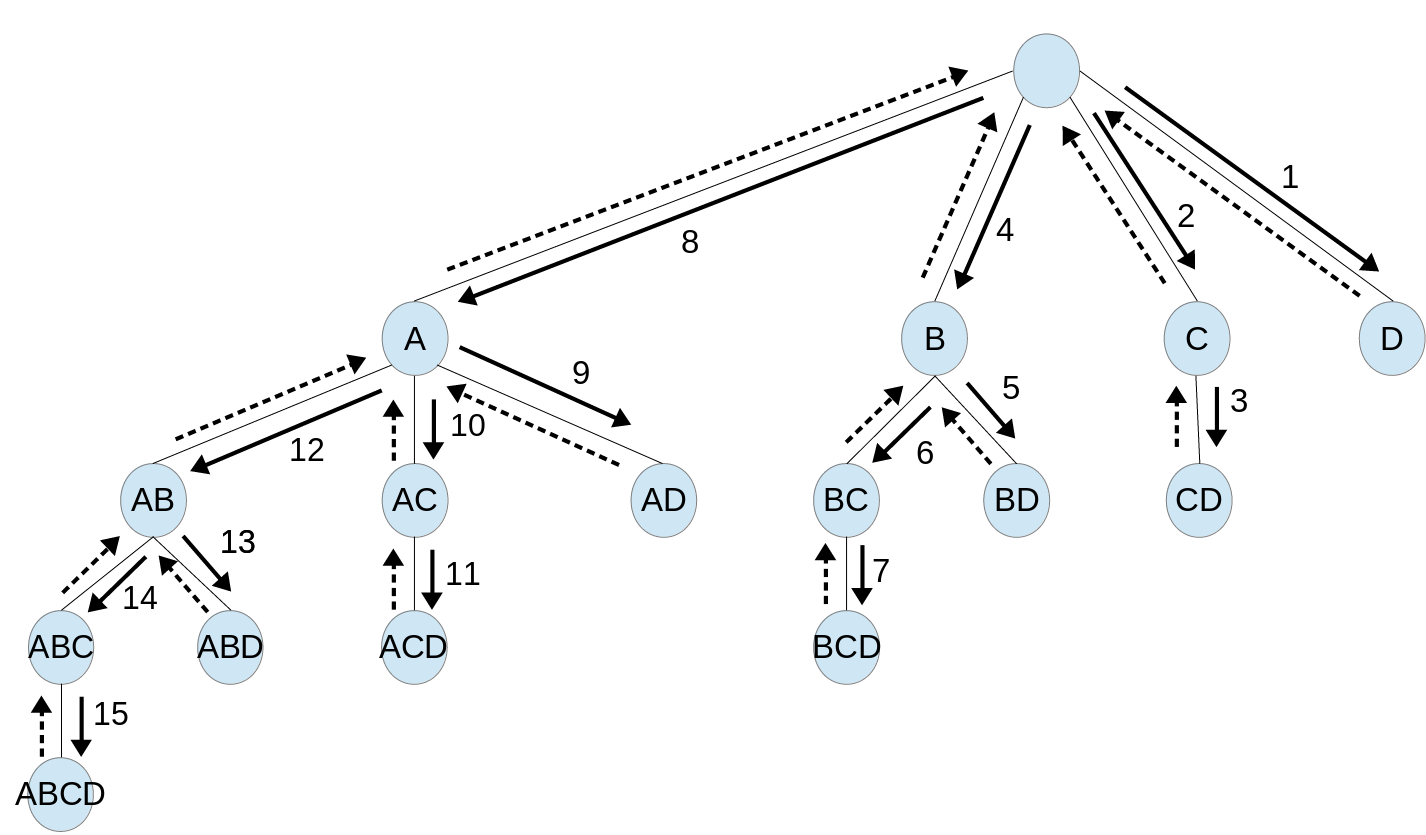
\includegraphics[width=1\textwidth]{figs/buscarecursiva}
\caption[Busca Recursiva.]
{Busca Recursiva.}
\label{fig:buscarecursiva}
\end{figure}

Um exemplo de como percorrer uma árvore com $m=4$ é apresentado na Figura \ref{fig:buscarecursiva}. Nesse exemplo, as setas sólidas representam as chamadas recursivas aos filhos dos vértices na árvore. Os números das arestas sólidas mostram a ordem em que as chamadas são feitas, ou seja, a ordem em que os vértices da árvore são visitados.

Quando a busca alcança uma folha ou quando um vértice da árvore já testou todos os seus filhos, sua instância do algoritmo é encerrada e a instância do seu pai é retomada. As setas tracejadas representam o retorno a um nível inferior da recursão sempre que uma instância em um vértice é encerrada. 

\begin{figure}[htb]
\centering
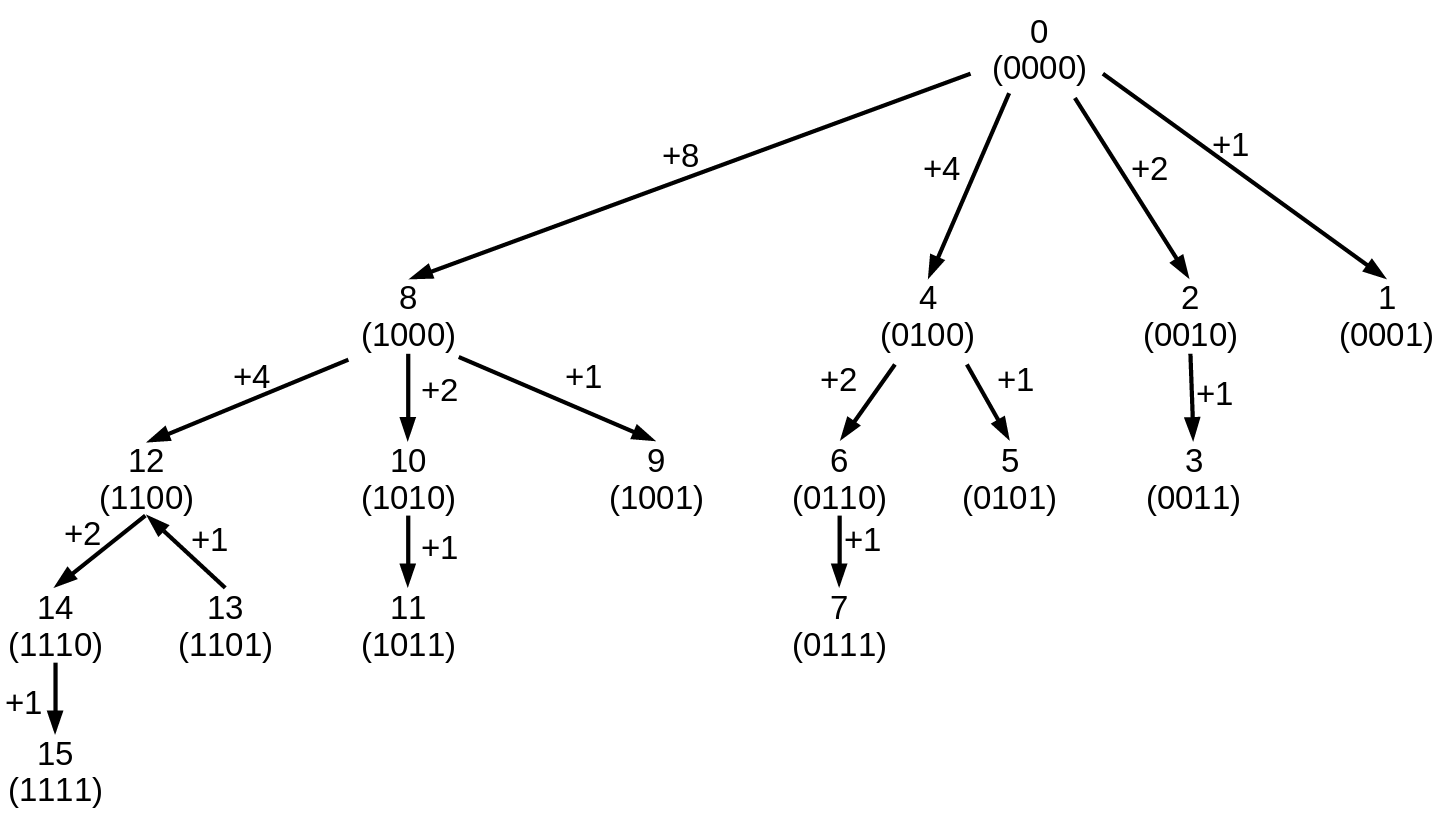
\includegraphics[width=1\textwidth]{figs/contagemrecursiva}
\caption[Contagem Recursiva.]
{Contagem Recursiva.}
\label{fig:contagemrecursiva}
\end{figure}

Na Figura \ref{fig:contagemrecursiva}, é mostrado, para a mesma árvore do exemplo anterior, como os vértices são alcançados. Somar $2^i$ a um conjunto codificado B, faz com que o {\it bit} $b_i$ seja alternado de 0 para 1, ou seja, inclui o enlace $e_i$ ao conjunto C. O valor de i é definido pelo índice do {\it bit} ativo menos signigicativo $b^*_i$. Como $B=0$ não tem {\it bits} ativos, então todos os seus {\it bits} podem ser variados.

Para cada vértice da árvore, uma pequena contagem é feita para variar o valor do indice i usado no incremento $2^i$ para ser somado ao próprio valor codificado do vértice e alcançar seus filhos. Essa contagem é definida de 0 até $i^*-1$. Por exemplo, na árvore da Figura \ref{fig:contagemrecursiva}, o vértice 8 possui $i^*=3$. Portanto possui 3 filhos e sua contagem será de 0 até 2, ou seja, seus filhos 9, 10, e 12 podem ser obtidos incrementando 8 de $2^0$, $2^1$ e $2^2$, respectivamente.

\section{“Podando” a Árvore de Combinações}

“Podar” uma árvore de combinações que esteja sendo percorrida usando o método da seção anterior é muito mais simples do que “saltar” em uma contagem. Quando uma folha $B' = B + 2^i$ na árvore é alcançada, como ela não tem filhos, a técnica não será mais aplicada e instância da busca que visitou tal folha é encerrada, de forma que a busca continua em $B''=B+2^i+1$. O mesmo acontece quando uma combinação $B'$ visitada não é viável. Nesse caso, mais uma vez devido a inviabilidade hereditária, todos os descendentes de $B'$ são ignorados e a busca continua em $B'$.

Dada essa situação, é importante ressaltar que, nem sempre irá existir um $B''$, ou seja, um vértice irmão de $B'$. Caso isso venha a acontecer, significa que todos os descendentes de $B$ já foram visitados (ou ignorados) e $B'$ é o último em seu ramo com altura $h$, ou seja, o último filho de $B$. Isso fará com que instância da recursão de $B$ se encerre e autoriza o seu pai na árvore a visitar algum outro filho (irmão de $B$), se houver. 

\section{Reaproveitando Cálculos}

No algoritmo anterior, era fundamental que houvesse um processo de decodificação do número $B$ em um conjunto $C$ para que os testes de interferência fossem realizados. No caso da busca recursiva, quando um novo vértice é visitado, o enlace $e_i$ correspondente ao índice $i$ do {\it bit} alternado é adicionado em $C$. Ao ser adicionado em $C$, a porção de interferência causada e sofrida por $e_i$ é atualizada. A viabilidade do conjunto $C$ é testada toda vez que um novo enlace é adicionado. Simetricamente, depois de visitar todos os seus descendentes, $e_i$ é removido de $C$.

Ao realizar o procedimento de adição e remoção dos enlaces descrito, dado um conjunto viável $B$, para testar a viabilidade de seus filhos na árvore, basta considerar a contribuição de interferência do enlace adicionado a $B$. Isso significa que todo o cálculo de SINR feito de 0 até $B$ não precisa ser refeito ao testar os filhos de $B$.

Além disso, a SINR já é calculada no momento em que um novo enlace é adicionado ao conjunto. Logo, para esse caso, a complexidade do algoritmo TIS é reduzida. Como as SINR já estão calculadas, basta iterar sobre os enlaces de $C$, fazendo a complexidade de tempo diminuir de $O(m^2)$ para $O(m)$. Como será detalhado no Capítulo \ref{cap:resultados}, o tempo do TIS também será reduzido para $O(m)$. Consequentemente, o algoritmo VIAVEL para o caso recursivo terá complexidade $O(m) + O(m) = O(m)$. 

\section{Algoritmo Recursivo para Enumeração de Conjuntos de Enlaces Viáveis}

Até o momento, uma nova ideia de como percorrer a árvore foi apresentada. Essa ideia permite que a árvore seja “podada” e dispensa a necessidade de decodificação, o que, intuitivamente, representa um ganho na complexidade de tempo em relação ao Algoritmo Iterativo. O Algoritmo Recursivo é apresentado a seguir.

\begin{algorithm}[h]
	\SetVline
	{\bf input:} Grafo direcionado $G=(V,E)$, Conjunto de Enlaces $C$, Inteiro $X$\\
	{\bf output:} Conjuntos de Enlaces Viáveis $F$\\
	\If{$X=0$}{
		\For{$i=0$ to $m-1$}{
			$RECURSIVO(G, C, X + 2^i)$\\
		}
	}
	\Else{
		$limite \leftarrow log2(X \& ~(X-1))$\\
		$C \leftarrow C \cup \{e_{limite}\}$\\
		\If{$VIAVEL(C)$}{
			$F \leftarrow F \cup {C}$\\
			\For{$i=0$ to $limite-1$}{
				$RECURSIVO(G, C, X + 2^i)$\\
			}
			$C \leftarrow C \ {e_{limite}}$\\
		}
	}
\caption{Algoritmo RECURSIVO}
\label{alg:recursivo}
\end{algorithm}

\subsubsection{Prova de Corretude}

Como mostrado na seção 4.2, se $X=0$, então toda a árvore é percorrida chamando o algoritmo RECURSIVO recursivamente para todos os descendentes. A condicional na linha 1 e 4 fazem o tratamento do caso especial em que $X=0$. A chamada recursiva da função só é feita quando o conjunto $C$ se mostra viável ou quando $limite>0$. Se $C$ não é viável então RECURSIVO não será chamada para seus descendentes, o que não problema devido a Inviabilidade Hereditária. Logo, ignorar os descendentes de uma combinação não viável não altera o resultado do algoritmo, apenas agiliza o processo. As linhas 6 e 11 garantem que qualquer enlace que seja adicionado a $C$ também seja removido. Finalmente, na linha 8, se $C$ é viável, então é adicionado ao conjunto $F$ e, por isso, $F$ contém todos os conjuntos de enlaces viáveis. Portanto, o algoritmo está correto.

\subsubsection{Análise da Complexidade}

Assim como no caso do algoritmo ITERATIVO, a complexidade de espaço é $O(m)$.

A complexidade de tempo desse algoritmo é parecida com a do algoritmo ITERATIVO. Contudo, como houveram algumas otimizações decorrentes do reaproveitamento dos cálculos da SINR, sua complexidade é um pouco menor. Houve uma redução de $O(|F|m^2)$ para $O(|F|m)$.

\section{Conclusão}

Apesar de uma concepção um pouco mais complexa, o algoritmo RECURSIVO obteve melhor complexidade de tempo em comparação com todas as técnicas apresentadas até agora. Tudo isso, devido a reutilização dos cálculos proporcionada por sua natureza recursiva. 
